\begin{tikzpicture}[x=1cm, y=1cm, font=\sffamily\footnotesize,
  ptitle/.style={anchor=west, font=\sffamily\bfseries\small, text=narrareddeep},
  textbox/.style={draw=phaseA!60, fill=phaseA!6, rounded corners=2pt, inner sep=4pt, anchor=north west,
                  align=left, font=\sffamily\scriptsize},
  lbl/.style={draw=#1, fill=white, fill opacity=0.9, text opacity=1, rounded corners=1pt, inner sep=1.6pt,
              line width=0.6pt, font=\sffamily\scriptsize},
  lblkey/.style={draw=#1, fill=white, fill opacity=0.95, text opacity=1, rounded corners=1pt, inner sep=1.8pt,
                 line width=1.0pt, font=\sffamily\scriptsize\bfseries},
  lead/.style={draw=#1, line width=0.7pt},
  path/.style={-{Latex[length=2.6mm, width=2.4mm]}, draw=black!85, line width=1.6pt},
  imgcap/.style={anchor=north, font=\sffamily\scriptsize, text=black!60},
  chip/.style={draw=black!30, fill=white, rounded corners=6pt, inner sep=2.5pt, font=\sffamily\footnotesize},
  flow/.style={-{Latex[length=1.6mm]}, draw=black!50, line width=0.6pt},
  lab/.style={anchor=east, font=\sffamily\footnotesize, text=black!75},
  txt/.style={anchor=west, font=\sffamily\footnotesize, text=black!75}]

\node[ptitle] at (0,0.000) {(a) The task and its room (AI2-THOR rendering of the benchmark trial)};
\node[textbox, text width=14.70cm] (obs) at (0,-0.280) {\textbf{Goal.} Your task is to: put two pillow in sofa.\\[1pt]\textbf{Initial observation.} You are in the middle of a room. Looking quickly around you, you see a armchair 1, a cabinet 4, a cabinet 3, a cabinet 2, a cabinet 1, a drawer 5, a drawer 4, a drawer 3, a drawer 2, a drawer 1, a dresser 1, a garbagecan 1, a safe 1, a shelf 12, a shelf 11, a shelf 10, a shelf 9, a shelf 8, a shelf 7, a shelf 6, a shelf 5, a shelf 4, a shelf 3, a shelf 2, a shelf 1, a sidetable 1, and a sofa 1.};
\begin{scope}[shift={($(obs.south west)+(0,-0.25)$)}]
\node[anchor=north west, inner sep=0] at (0.000,0.000) {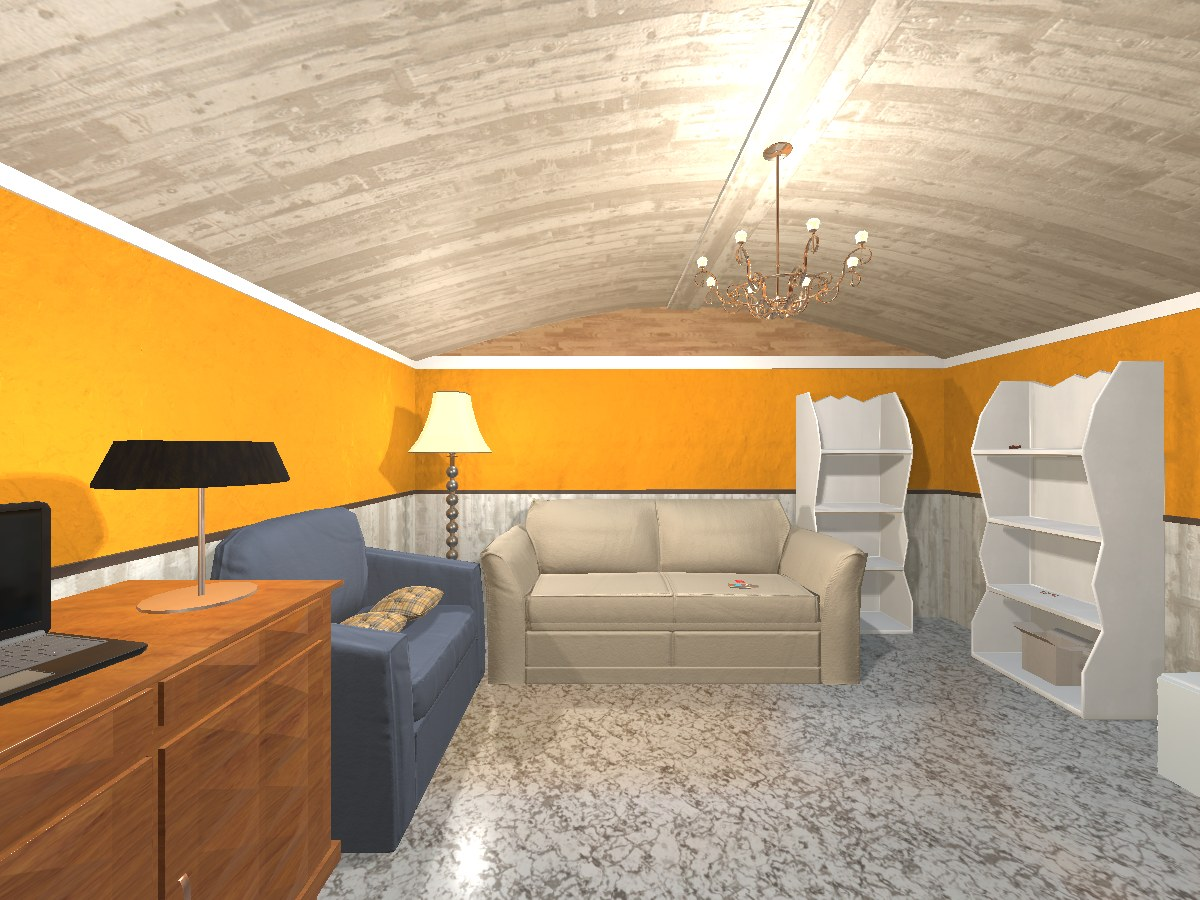
\includegraphics[width=7.919cm]{figures/cases/task2_view1.jpg}};
\draw[black!35, line width=0.4pt] (0.000,0.000) rectangle ++(7.919,-5.939);
\draw[dimF, line width=1.1pt] (2.462,-4.108) circle (0.261);
\draw[lead=dimF] (2.462,-4.108) -- (2.462,-3.608);
\fill[dimF] (2.462,-4.108) circle (0.06);
\node[lblkey=dimF] at (2.462,-3.608) {pillow};
\draw[dimF, line width=1.1pt] (2.683,-3.986) circle (0.289);
\draw[lead=dimF] (2.683,-3.986) -- (1.833,-4.177);
\fill[dimF] (2.683,-3.986) circle (0.06);
\node[lblkey=dimF] at (1.833,-4.177) {pillow};
\draw[dimA, line width=1.1pt, rounded corners=1pt] (1.386,-3.352) rectangle (3.201,-5.629);
\draw[lead=dimA] (2.293,-4.491) -- (2.293,-4.991);
\fill[dimA] (2.293,-4.491) circle (0.06);
\node[lblkey=dimA] at (2.293,-4.991) {armchair: the pillows are here};
\draw[liftpositive, line width=1.1pt, rounded corners=1pt] (3.168,-3.293) rectangle (5.722,-4.521);
\fill[liftpositive] (4.445,-3.907) circle (0.06);
\node[lblkey=liftpositive] at (4.445,-3.907) {sofa: put both here};
\draw[lead=black!55] (1.132,-4.887) -- (0.751,-4.148);
\fill[black!55] (1.132,-4.887) circle (0.06);
\node[lbl=black!45] at (0.751,-4.148) {dresser};
\fill[black!55] (7.045,-3.570) circle (0.06);
\node[lbl=black!45] at (7.045,-3.570) {shelves};
\draw[lead=black!55] (1.584,-5.085) -- (1.584,-4.585);
\fill[black!55] (1.584,-5.085) circle (0.06);
\node[lbl=black!45] at (1.584,-4.585) {cabinets};
\draw[lead=black!55] (0.505,-5.012) -- (0.771,-5.474);
\fill[black!55] (0.505,-5.012) circle (0.06);
\node[lbl=black!45] at (0.771,-5.474) {drawers};
\node[anchor=north west, inner sep=0] at (8.169,0.000) {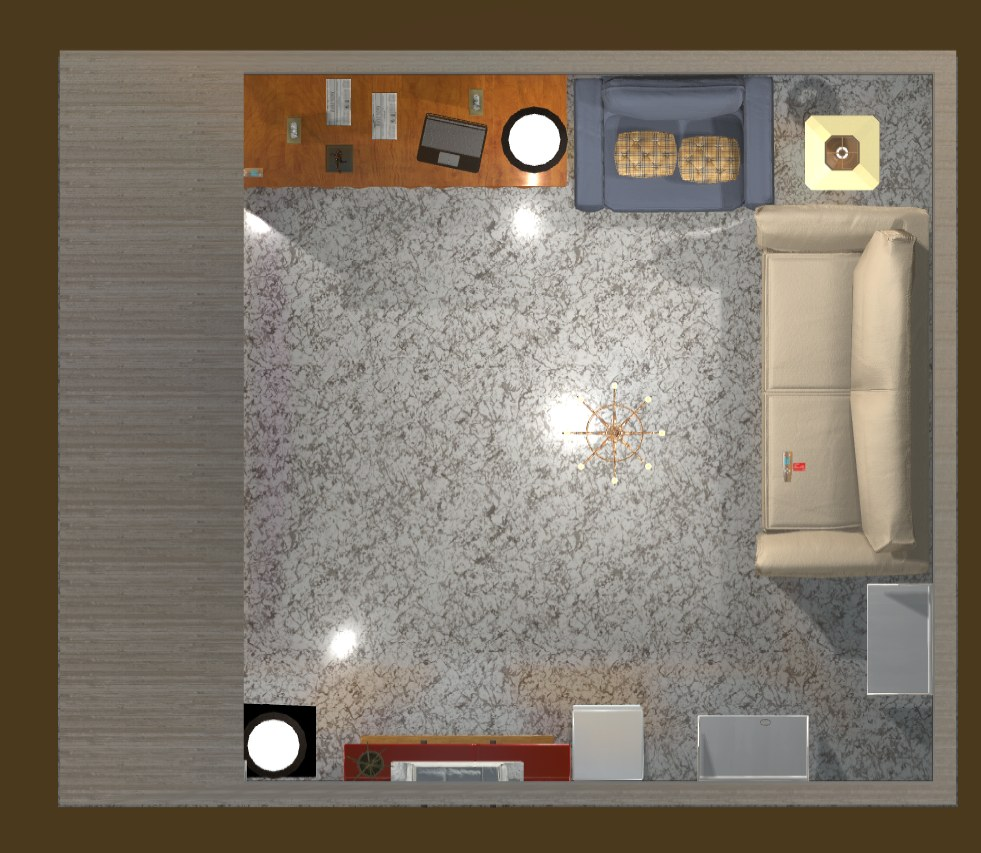
\includegraphics[width=6.831cm]{figures/cases/task2_map.jpg}};
\draw[black!35, line width=0.4pt] (8.169,0.000) rectangle ++(6.831,-5.939);
\fill[black, opacity=0.22] (10.468,-2.234) -- ++(-45:1.1) arc (-45:45:1.1) -- cycle;
\fill[black] (10.468,-2.234) circle (0.08);
\draw[white, line width=3.4pt, opacity=0.85] (12.967,-1.160) -- (13.815,-2.515);
\draw[path] (12.967,-1.160) -- (13.815,-2.515);
\draw[lead=dimA] (12.861,-0.991) -- (12.861,-0.491);
\fill[dimA] (12.861,-0.991) circle (0.06);
\node[lblkey=dimA] at (12.861,-0.491) {armchair: the pillows are here};
\draw[lead=liftpositive] (13.948,-2.727) -- (13.578,-2.265);
\fill[liftpositive] (13.948,-2.727) circle (0.06);
\node[lblkey=liftpositive] at (13.578,-2.265) {sofa: put both here};
\draw[lead=black!55] (10.471,-1.290) -- (10.195,-0.828);
\fill[black!55] (10.471,-1.290) circle (0.06);
\node[lbl=black!45] at (10.195,-0.828) {cabinets};
\draw[lead=black!55] (12.003,-1.290) -- (11.393,-0.936);
\fill[black!55] (12.003,-1.290) circle (0.06);
\node[lbl=black!45] at (11.393,-0.936) {cabinet};
\draw[lead=black!55] (11.139,-1.191) -- (10.239,-1.383);
\fill[black!55] (11.139,-1.191) circle (0.06);
\node[lbl=black!45] at (10.239,-1.383) {drawers};
\draw[lead=black!55] (9.982,-1.191) -- (9.028,-1.191);
\fill[black!55] (9.982,-1.191) circle (0.06);
\node[lbl=black!45] at (9.028,-1.191) {drawer};
\draw[lead=black!55] (9.700,-5.087) -- (9.700,-4.587);
\fill[black!55] (9.700,-5.087) circle (0.06);
\node[lbl=black!45] at (9.700,-4.587) {drawer};
\draw[lead=black!55] (10.851,-0.908) -- (10.029,-0.342);
\fill[black!55] (10.851,-0.908) circle (0.06);
\node[lbl=black!45] at (10.029,-0.342) {dresser};
\draw[lead=black!55] (8.937,-1.418) -- (8.937,-1.918);
\fill[black!55] (8.937,-1.418) circle (0.06);
\node[lbl=black!45] at (8.937,-1.918) {garbagecan};
\draw[lead=black!55] (12.402,-5.188) -- (12.402,-4.688);
\fill[black!55] (12.402,-5.188) circle (0.06);
\node[lbl=black!45] at (12.402,-4.688) {safe};
\draw[lead=black!55] (13.917,-4.839) -- (13.917,-4.339);
\fill[black!55] (13.917,-4.839) circle (0.06);
\node[lbl=black!45] at (13.917,-4.339) {shelves};
\draw[lead=black!55] (9.487,-5.379) -- (8.877,-5.025);
\fill[black!55] (9.487,-5.379) circle (0.06);
\node[lbl=black!45] at (8.877,-5.025) {shelves};
\draw[lead=black!55] (9.700,-5.189) -- (9.031,-5.542);
\fill[black!55] (9.700,-5.189) circle (0.06);
\node[lbl=black!45] at (9.031,-5.542) {sidetable};
\node[imgcap] at (3.960,-5.979) {first-person view inside the room};
\node[imgcap] at (11.585,-5.979) {the room from above; cone: the left view; arrow: the expert's route};
\node[anchor=west, font=\sffamily\bfseries\footnotesize, text=black!70] at (0,-6.739) {Expert solution (8 steps):};
\node[chip, anchor=west] (s0) at (3.900,-6.739) {go to armchair};
\node[chip, anchor=west] (s1) at (6.588,-6.739) {take pillow from armchair};
\draw[flow] (s0.east) -- (s1.west);
\node[chip, anchor=west] (s2) at (10.838,-6.739) {go to sofa};
\draw[flow] (s1.east) -- (s2.west);
\node[chip, anchor=west] (s3) at (3.900,-7.239) {move pillow to sofa};
\node[chip, anchor=west] (s4) at (7.298,-7.239) {go to armchair};
\draw[flow] (s3.east) -- (s4.west);
\node[chip, anchor=west] (s5) at (9.986,-7.239) {take pillow from armchair};
\draw[flow] (s4.east) -- (s5.west);
\node[chip, anchor=west] (s6) at (3.900,-7.739) {go to sofa};
\node[chip, anchor=west] (s7) at (6.020,-7.739) {move pillow to sofa};
\draw[flow] (s6.east) -- (s7.west);
\node[ptitle] at (0.000,-8.539) {(b) What happened: \texttt{GPT-4o-mini}, seed 0};
\node[lab] at (1.650,-9.139) {expert};
\fill[black!30, rounded corners=1pt] (1.750,-8.989) rectangle ++(1.600,-0.3);
\node[txt] at (3.430,-9.139) {8};
\node[lab] at (1.650,-9.599) {no memory};
\fill[phaseA!35, rounded corners=1pt] (1.750,-9.449) rectangle ++(6.000,-0.3);
\node[txt] at (7.830,-9.599) {30, not solved};
\node[lab] at (1.650,-10.059) {memory};
\fill[salmon!60, rounded corners=1pt] (1.750,-9.909) rectangle ++(6.000,-0.3);
\node[txt] at (7.830,-10.059) {30, not solved};
\draw[densely dashed, black!40] (7.750,-8.889) -- (7.750,-10.319);
\node[font=\sffamily\scriptsize, text=black!50, anchor=north] at (7.750,-10.319) {30-step limit};
\node[txt] at (10.600,-9.139) {prompt tokens: 89,011 $\rightarrow$ 109,495};
\node[txt] at (10.600,-9.559) {effect over 3 demo pairs:};
\node[txt] at (10.600,-9.979) {\quad not reported for this task};
\end{scope}
\end{tikzpicture}
